\chapter{Introducción}
\label{cap:introduccion}
\setcounter{page}{1}

En la última década, la evolución tecnológica ha provocado una transformación radical en nuestra forma de vivir, trabajar y relacionarnos desempeñando la tecnología un papel 
fundamental en el avance de la sociedad e impulsando una serie de innovaciones que se extienden desde la invención de la rueda hasta la era digital contemporánea. 
Por ejemplo, los ordenadores empezaron siendo grandes máquinas que ocupaban habitaciones enteras que requerían una gran cantidad de energía y mantenimiento. Hoy en día, los ordenadores
son dispositivos ligeros y eficientes que pueden realizar múltiples cálculos por segundo. La telefonía móvil también ha experimentado una evolución destacada, los primeros móviles
se caracterizaban de ser dispositivos pesados y grandes que solo podían realizar llamadas, pero hoy en día no solamente podemos realizar llamadas telefónicas con un teléfono móvil,sino 
que también podemos enviar mensajes, navegar por internet, tomar fotos, escuchar música, ver vídeos y mucho más. \newline

Entre las diversas ramas de la tecnología, la robótica se destaca como una de las más prometedoras. Apareciendo como disciplina durante la década de los años 60, teniendo un crecimiento exponencial en las últimas décadas. Dos figuras clave en el desarrollo de la robótica fueron Jorge Devalo (1921-2011) y 
José Engarberare (1925-2015) considerados como padres de la robótica, quienes crearon el brazo robótico llamado Unimate \footnote{\url{https://robotsguide.com/robots/unimate/}}. 
Este brazo robótico de 6 grados de libertad (3 grados en el brazo y 3 grados en la muñeca) estaba construido con una base de acero y aluminio en su brazo, 
constaba de sensores rotatorios personalizados que permitian al robot poder conocer la posición de sus articulaciones y así controlar
sus movimientos de manera eficiente y actuadores hidráulicos. Gracias a este robot las fabricas de producción empezaron a ser automatizadas facilitando la creación 
de otro tipo de robots industriales dando lugar al inicio de una nueva en el mundo industrial.

\begin{figure} [H]
  \begin{center}
    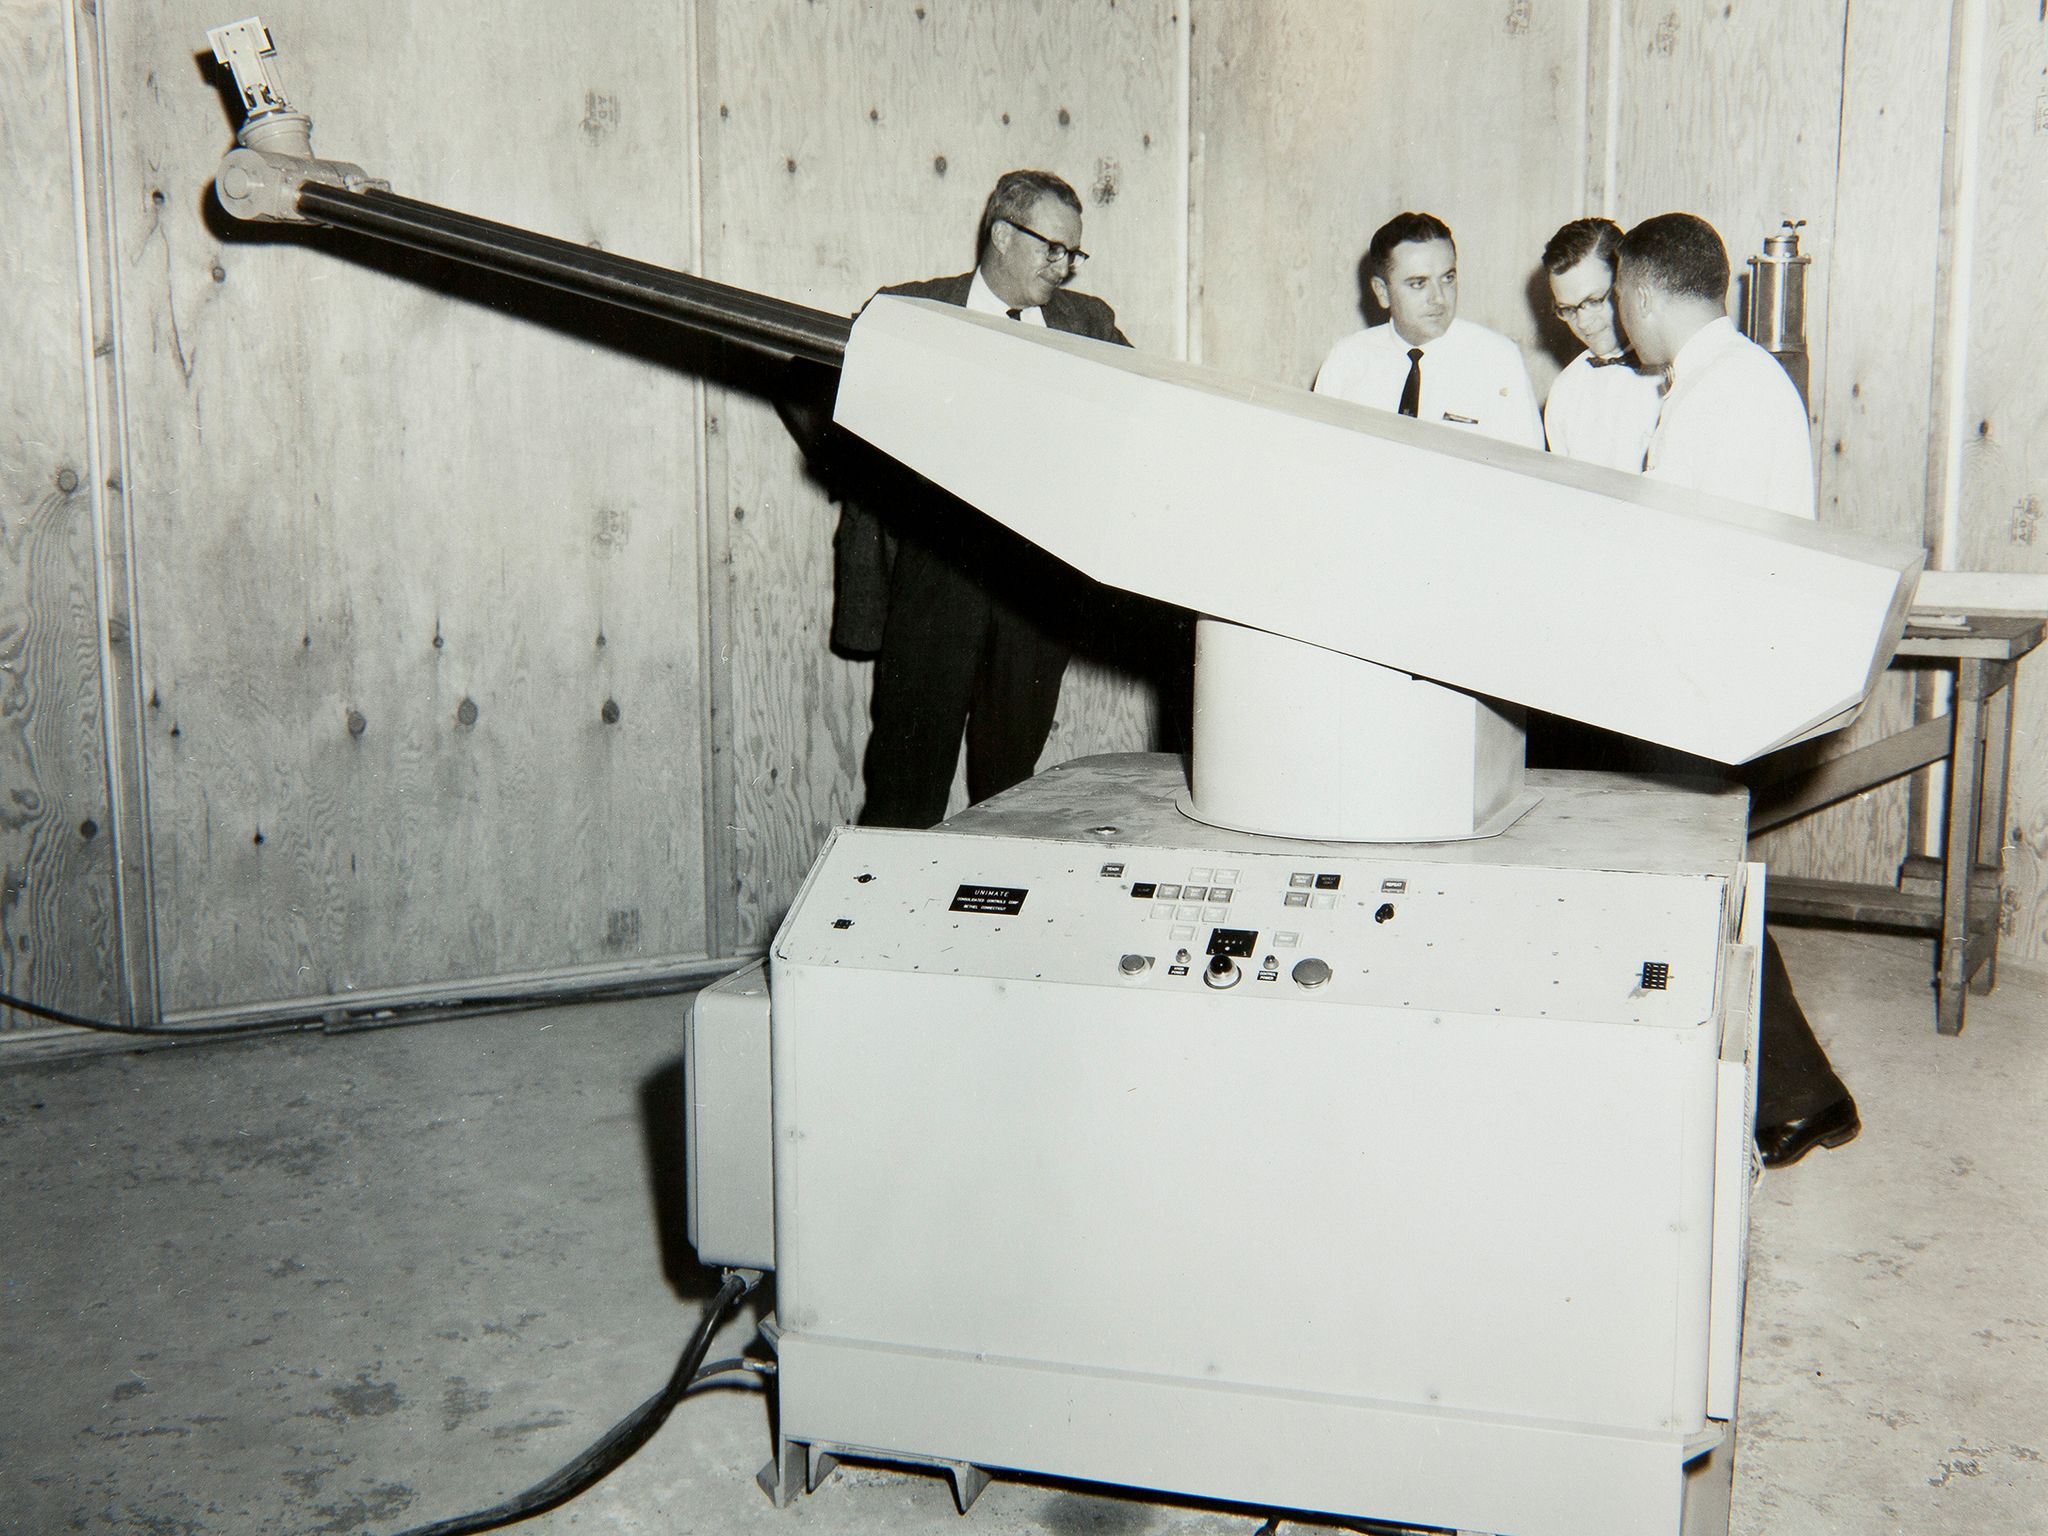
\includegraphics[scale=0.15]{figs/introducción/Unimate.jpg}
  \end{center}
  \caption{Unimate}
  \label{fig:unimate}
\end{figure}\
\newline 
\newline 

La robótica ha tenido un cambio asombroso desde la creación del robot Unimate, pasando de ser simples máquinas programables a sistemas inteligentes capaces de aprender y adaptarse 
a su entorno teniendo avances en diversas disciplinas de la ingeniería, como la informática, la inteligencia artificial, la ingenieria de control, la mecánica y otras más. 
Los robots de hoy en día no solo tienen la capacidad de realizar tareas programadas y repetitivas, sino que también tienen la capacidad de interactuar con su entorno
, tomar decisiones basadas en la información sensorial y aprender de sus experiencias. Este avance en la robótica nos ha permitido tener una definición más precisa de lo que es 
la robótica moderna, definiendo la robótica como ciencia interdisciplinaria encargada de la creación, funcionamiento, estructuración, fabricación y uso de los robots. 
Esta definición mencionada incluye no solo los componentes mecánicos y eléctricos, sino que también los algoritmos que los controlan, los sensores que les permiten recopilar
datos de su entorno y los sistemas que procesan esta información y toman decisiones.

\begin{figure} [H]
  \begin{center}
    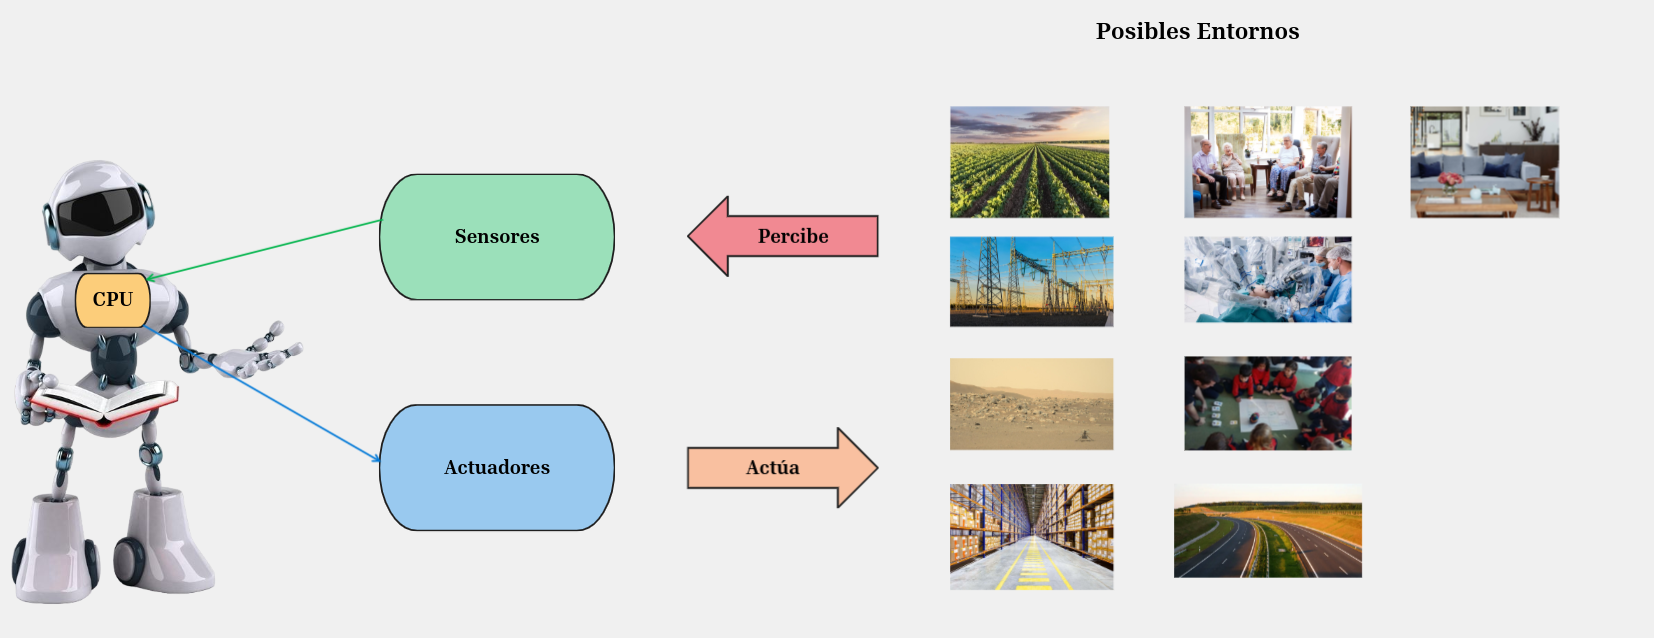
\includegraphics[scale=0.25]{figs/introducción/robot.png}
  \end{center}
  \caption{Definición de robot.}
  \label{fig:robot}
\end{figure}\

Lo que hace que un robot tenga la capacidad de aprender y adaptarse a un entorno abierto de nuevas oportunidades para la robótica, como la medicina, la exploración
lunar, la asistencia personal, la automatización industrial y más. Además de abrir nuevas aplicaciones y tareas como puede ser la navegación autónoma, la detención de objetos o 
la manipulación de objetos con sensores táctiles y de fuerza, dichas tareas pueden realizar pueden ser peligrosas, delicadas, sucias o monótonas 
(conocidas como las 4D's: dull,dirty, dangerous and dear) \footnote{:\url{https://www.forbes.com/sites/bernardmarr/2017/10/16/the-4-ds-of-robotization-dull-dirty-dangerous-and-dear/?sh=40bb6cec3e0d}}

\section{Enfoques en la robótica}
\label{sec:enfoquesrobotica} % etiqueta para luego referenciar esta sección

A lo largo de la evolución de la robótica, han surgido dos enfoques fundamentales para el diseño y la operación de robots, cada uno de estos enfoques presentan diferentes
formas de interactuar y operar robots,con sus propias caracteristicas y aplicaciones únicas. 

\subsection{Teleoperación}
\label{sec:subseccion}

La teleoperación surge de la necesidad de manipular objetos o realizar tareas en entornos complejos, peligrosos y distantes para el ser humano. Desde la historia, el ser humano
ha utilizado una variedad de herramientas para ampliar su capacidad de manipulación como palos utilizados para caer la fruta madura de un arbol. Con el tiempo, se desarrollaron 
dispositivos más complejos, como pinzas que permitían manipular piezas o alcanzar objetos de díficil acceso facilitando el trabajo para el operario. En la era moderna, la teleoperación
ha estado evolucionando hasta el punto de incluir sistemas robóticos robustos que pueden ser controlados a distancia, permitiendo al operario poder realizar
tareas en entornos peligrosos e innacesibles para el ser humano como puede ser la exploración espacial, la cirugía de un ser humano u inspección nuclear. \newline

La intervencción del operador humano en los sistemas de teleoperación de robots es imprescendible, debe ser capaz de poder intepretar los datos sensoriales que proporciona el robot, así como de 
tomar decisiones robustas y precisas dependiendo de la situación. Esto conlleva tener una capacidad de realizar múltiple tareas simultáneamente, adaptarse a situaciones imprevistas. \newline

Hoy en día, la teleoperación de robots tiene variedad de aplicaciones. Una de ellas puede ser la exploración espacial, en donde se utiliza la teleoperación
como técnica de manipulación remota como el Sojourner Rover. El Sojourner Rover\footnote{\url{https://www.astronomy.com/space-exploration/sojourner-nasas-first-mars-rover/}} 
es un pequeño robot móvil compuesto por 6 ruedas creado por los cientificos de la NASA para estudiar 
la superficie de Marte con la capacidad de enviar imagenes en directo y realizar analisis del terreno del planeta. Gracias a sus ruedas podía moverse por terrenos rocosos y de dificil acceso
ya que estaban equipadas materiales como de aluminio y acero inoxidable. \newline

\begin{figure} [H]
  \begin{center}
    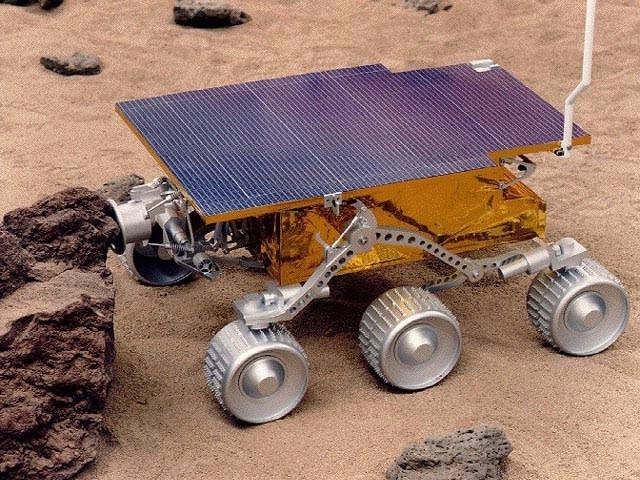
\includegraphics[scale=0.4]{figs/introducción/Sojourner.jpg}
  \end{center}
  \caption{Sojourner Rover}
  \label{fig:Sojourner}
\end{figure}\

\newpage
Con esta misión espacial se pudo probar como era el entorno marciano con técnicas realizadas en los laboratorios de la NASA demostrando que se podia realizar una teleoperación en 
el espacio abriendo el camino a futuros rovers como el Spirit, Opportunity y más \footnote{\url{https://spaceplace.nasa.gov/mars-spirit-opportunity/sp/}}. 

\subsection{Autonomía}
\label{sec:subseccion}

La robótica autónoma consiste en tener robots que sean capaces de operar y realizar tareas de forma independiente sin la intervencción de un ser humano. En contraste con los 
robots teleoperados, este tipo de robots necesitan un comportamiento más robusto y preciso para realizar tareas independientes basandose en la percepción del entorno 
y en la toma de decisiones autónomas. \newline

El concepto de automía en los sistemas robóticos se esta convirtiendo en un area de investigación activa y en rápido desarrollo. Los avances en inteligencia artificial (IA), visión 
artificial, aprendizaje automático han facilitado la creación de robots autonómos capaces de llevar a acbo amplias variedades de tareas en entornos no estructurados y cambiantes. 

\subsubsection{Los robots móviles}
\label{sec:subseccion}


\subsubsection{La condución autónoma}
\label{sec:subseccion}

\subsubsection{Robótica aérea}
\label{sec:subseccion}

Dentro del campo de la robótica aérea tenemos los drones. Podemos definir un dron, como vehículo aéreo no tripulado (UAV), es un tipo de aeronave que puede operar sin la 
necesidad de un piloto humano a bordo. Estos dispositivos pueden ser controlados remotamente por un operador humano o navegar autonomamente incoporando software 
en su sistema. \newline

El origen de los drones se remonta a la Primera Guerra Mundial con el biplano Kettering Bug.
Este era un torpedo no tripulado de 240 kg (con una envergadura de 4,5 m, una longitud de
3,8 m y una altura de 2,3 m)\footnote{\url{https://www.nationalmuseum.af.mil/Visit/Museum-Exhibits/Fact-Sheets/Display/Article/198095/kettering-aerial-torpedo-bug/}} era propulsado por un motor alternativo. Podía volar de
forma autónoma hasta un punto específico, donde soltaba sus alas y caía en “caída libre” \footnote{\url{https://daytonunknown.com/2023/06/30/the-kettering-bug-the-worlds-first-drone/}}.\newline

Avanzando en la historia, en 1935 se desarrolló el DH.82 Queen Bee\footnote{\url{https://dronewars.net/2014/10/06/rise-of-the-reapers-a-brief-history-of-drones/}}. Este era un blanco aéreo sin piloto que era controlado por radio. De hecho, parece que el término “dron” se originó a partir del nombre, que se refiere a la abeja macho que realiza un vuelo en busca de la abeja reina y luego fallece. \newline

Durante la Segunda Guerra Mundial, quizás el más conocido fue el V-1 "Flying Bomb"\footnote{\url{https://migflug.com/jetflights/the-v1-flying-bomb/}} , el primer misil
de crucero operativo del mundo, en donde su sistema de guía prestablecido incluía una brújula magnética que monitoreaba un autopiloto con giroscopios. También en este periodo, destacaremos el \textit{Proyect Aphrodite} \cite{Aphrodite}, fue un programa que tenía como objetivo convertir bombarderos en bombas voladoras no tripuladas que eran controladas por radio. Más adelante estos bombarderos no tripulados se utilizaron para volar a traves de nubes de hongo
después de las pruebas nucleares. \newline

Destacando más UAVs, tenemos la familia Teledyne Ryan Firebee/Firefly \footnote{\url{https://www.designation-systems.net/dusrm/m-34.html}}, estos sistemas generalmente se lanzaban desde el aire y se recuperaban mediante una combinación de paracaidas y helicopteros. El Lockheed D-21 fue uno de los sistemas más impresionantes durante la Guerra Fría. Este UAV fue propulsado por estatorreactor con velocidades mayores que Mach 3 \footnote{\url{https://www.marchfield.org/aircraft/unmanned/d-21-drone-lockheed/}} . En la Edad Moderna, destacamos El Condor \cite{CondorUAV}, fue el primer UAS en utilizar navegación GPS y tecnología de aterrizaje automático y el Predactor \footnote{\url{https://www.airforce-technology.com/projects/predator-uav/?cf-view}}. 
En la época dorada, gracias a los avances anteriores se pudo desarrollar sistemas militares esenciales que han demostrado su valor y el desarrollo de vehículos aéreos no tripulados pequeños (small UAV). Este ultimo ha despertado un gran interés significativo resaltando como puntos de entrega al mercado civil. \newline

\begin{figure}[H]
  \begin{center}
    \subfigure[Kettering Bug]{
     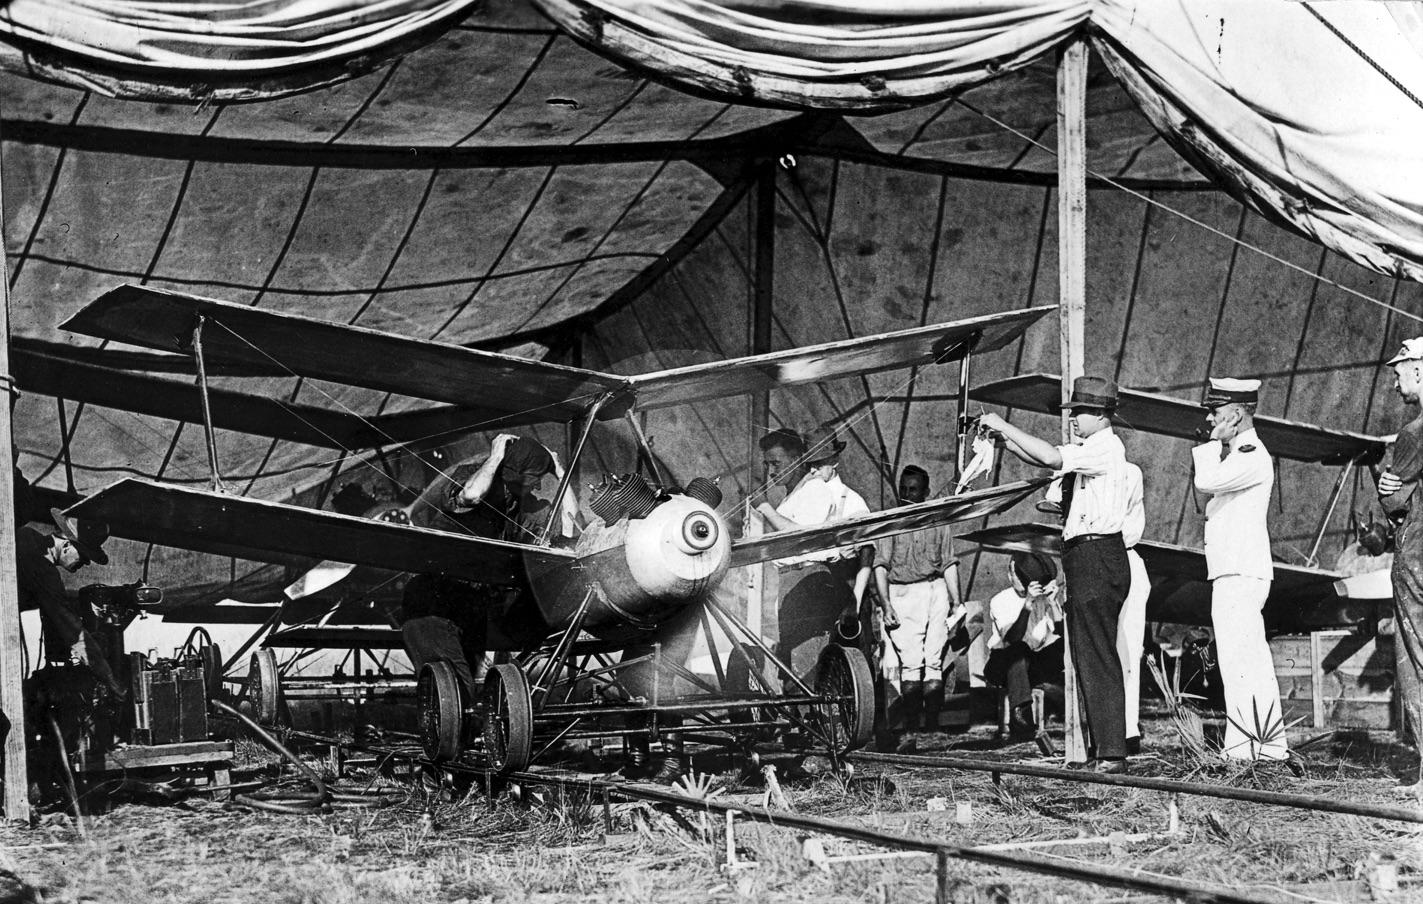
\includegraphics[width=0.3\textwidth,height=0.2\textwidth ]{figs/introducción/historia_drones/kettering-bug.jpg}
     \label{f:Kettering Bug}}
    \subfigure[Queen Bee]{
     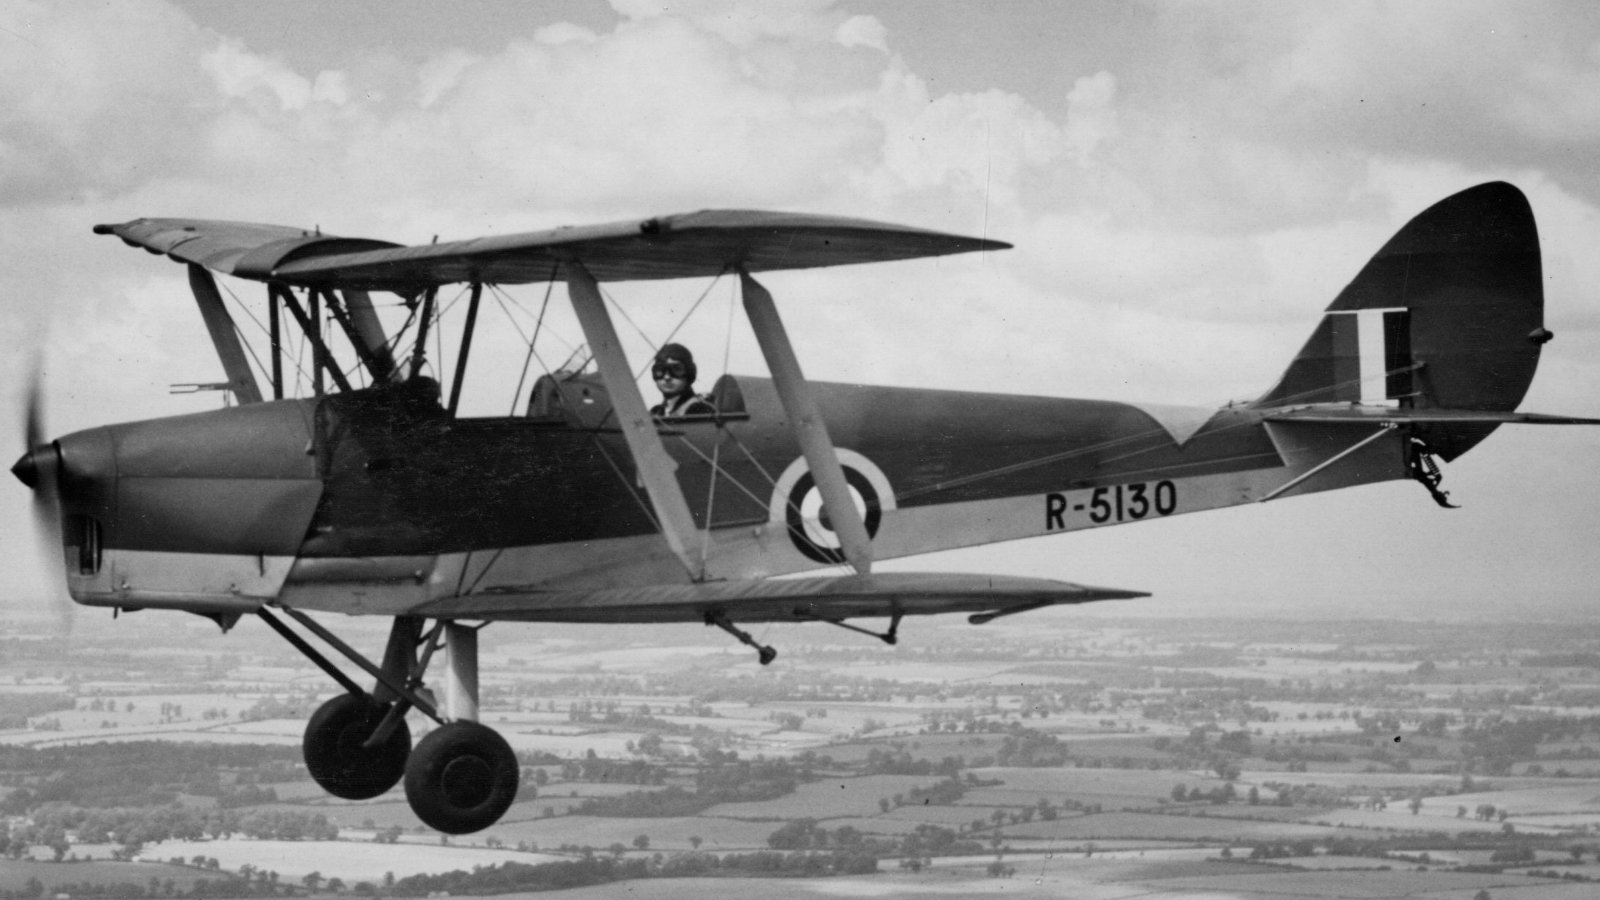
\includegraphics[width=0.3\textwidth,height=0.2\textwidth ]{figs/introducción/historia_drones/queen-bee.jpg}
     \label{f:Queen Bee}}
    \subfigure[V-1]{
      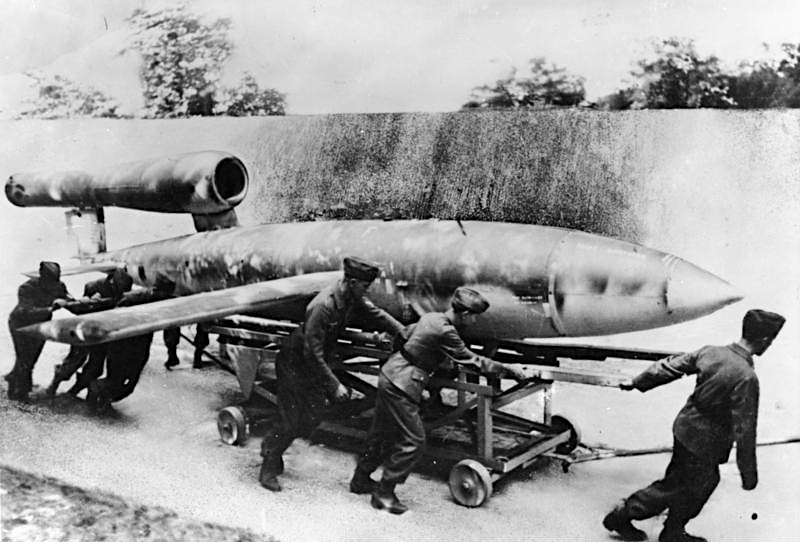
\includegraphics[width=0.3\textwidth,height=0.2\textwidth ]{figs/introducción/historia_drones/V-1.jpg}
      \label{f:V-1 "Flying Bomb"}}
    \subfigure[Proyect Aphrodite]{
      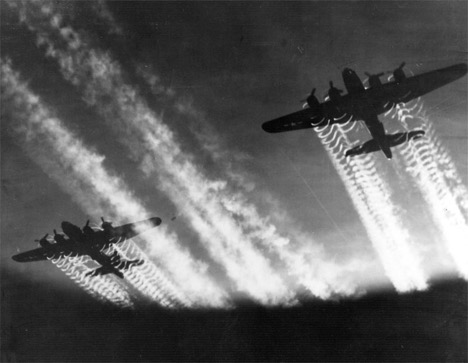
\includegraphics[width=0.3\textwidth,height=0.2\textwidth ]{figs/introducción/historia_drones/proyect-aphorite.jpg}
      \label{f:Proyect Aphrodite"}}
    \subfigure[Teledyne Ryan Firebee/Firefly]{
      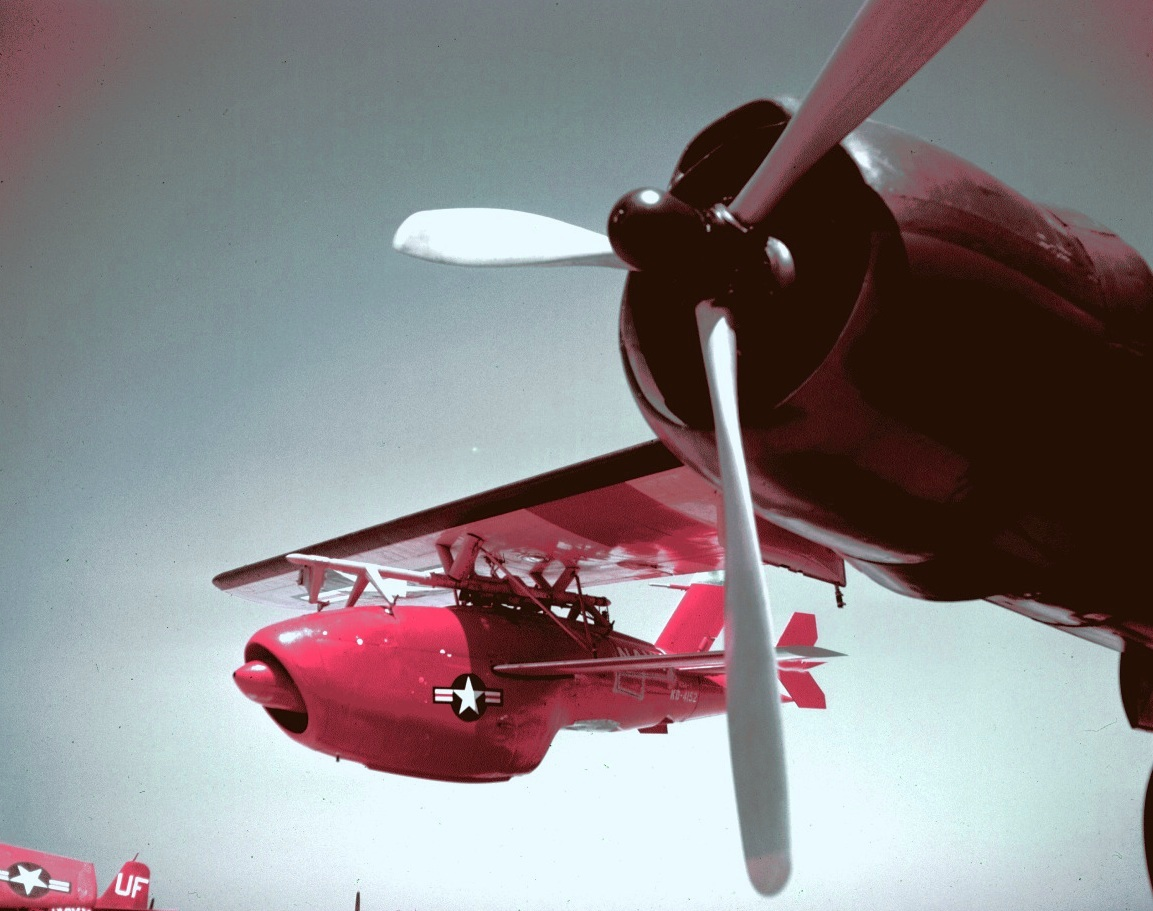
\includegraphics[width=0.3\textwidth,height=0.2\textwidth ]{figs/introducción/historia_drones/Firebee.jpg}
      \label{f:Teledyne Ryan Firebee/Firefly"}}
    \subfigure[Lockheed D-21]{
      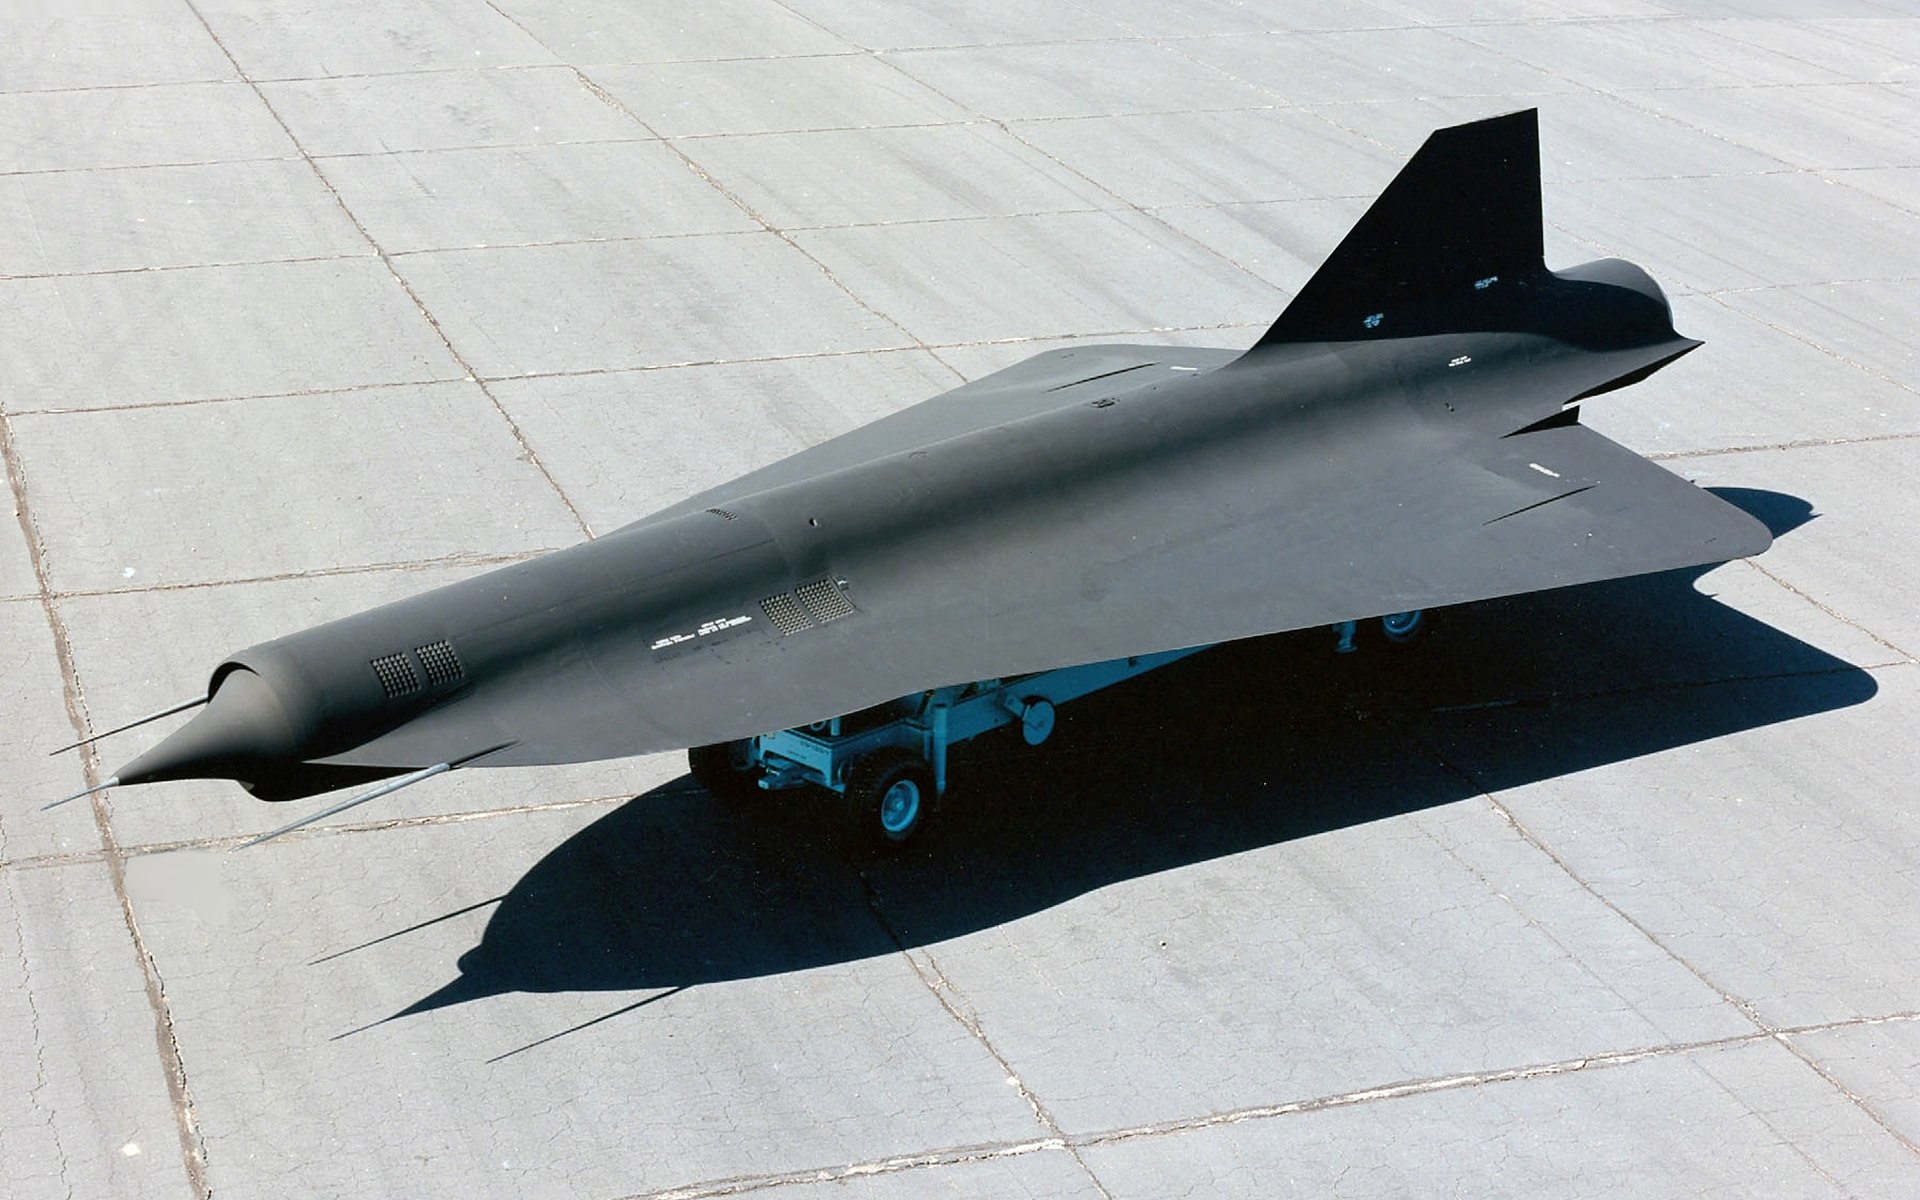
\includegraphics[width=0.3\textwidth,height=0.2\textwidth ]{figs/introducción/historia_drones/The_Lockheed_D-21.jpg}
      \label{f:Lockheed D-21"}}
    \subfigure[El Condor]{
      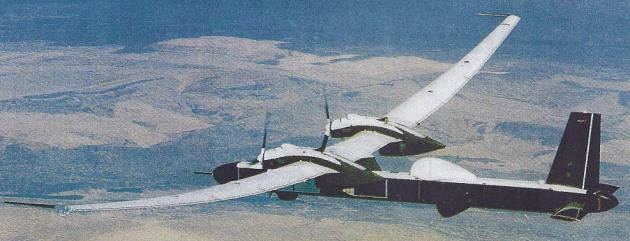
\includegraphics[width=0.3\textwidth,height=0.2\textwidth ]{figs/introducción/historia_drones/Boeing-Condor-UAV-23.png}
      \label{f:El Condor"}}
    \subfigure[Small UAV]{
      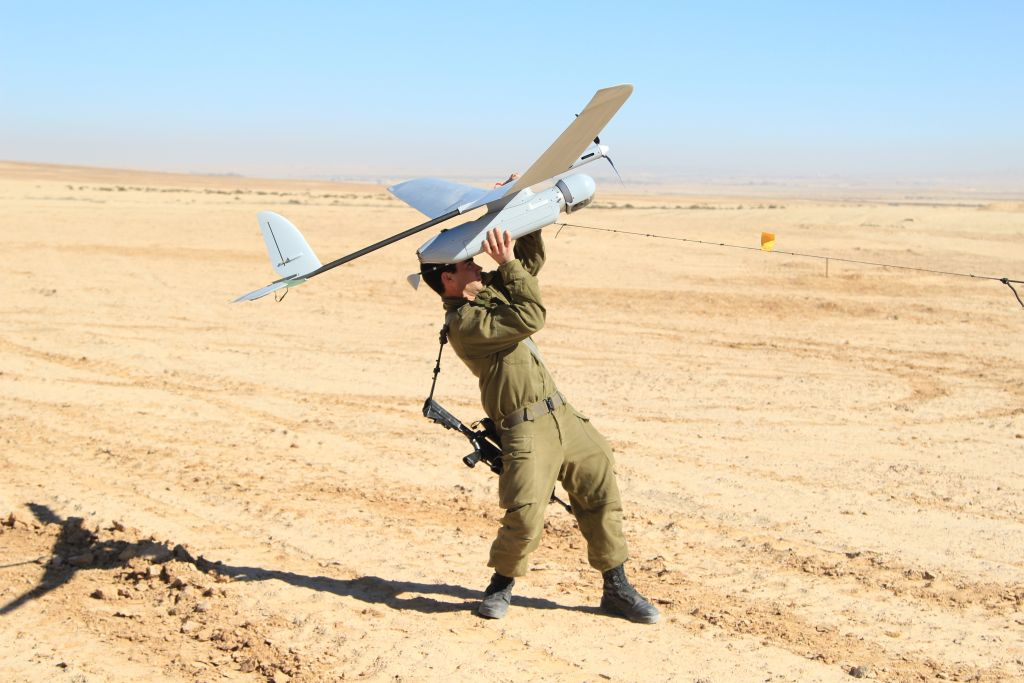
\includegraphics[width=0.3\textwidth,height=0.2\textwidth ]{figs/introducción/historia_drones/small-UAV.jpg}
      \label{f:small-UAV"}}
    \subfigure[Dron]{
      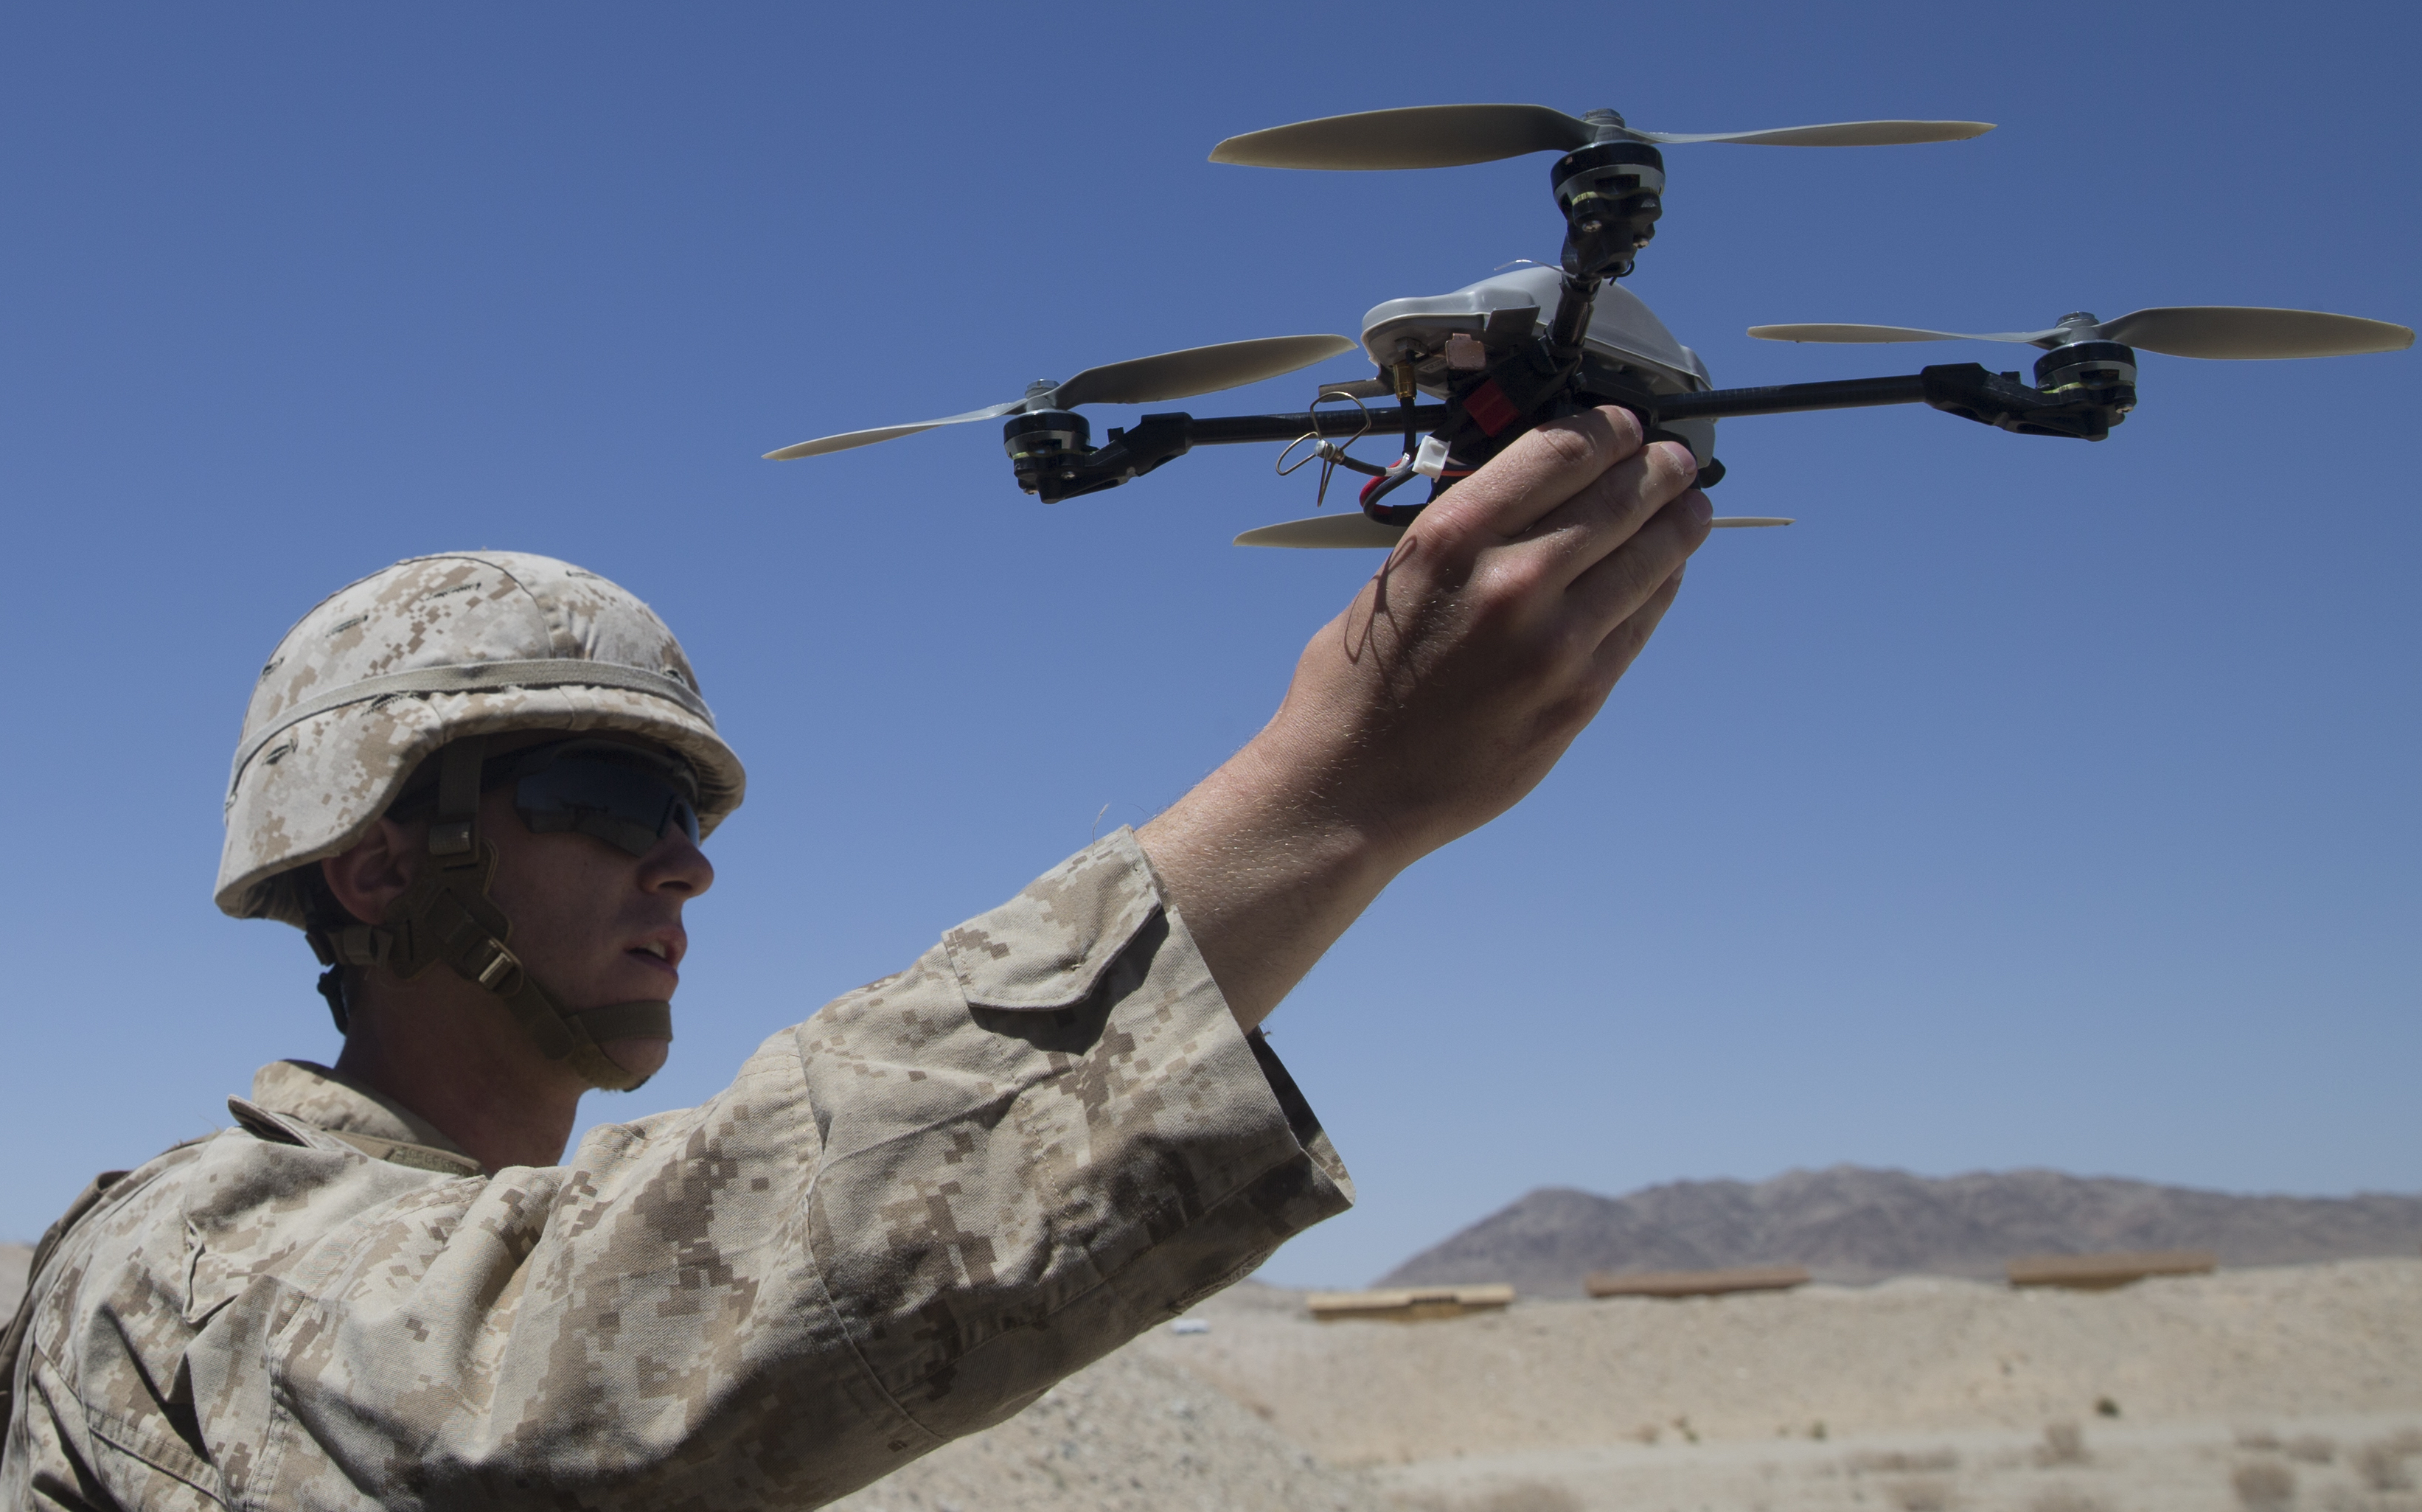
\includegraphics[width=0.3\textwidth,height=0.2\textwidth ]{figs/introducción/historia_drones/dron.jpg}
      \label{f:dron"}}
  \caption{Historia de los drones}
  \label{f:Drones}
  \end{center}
 \end{figure}

 En la actualidad, la industria de los drones sigue evolucionando a un ritmo exponencial teniendo 

\newpage
\section{Aplicaciones de drones dentro del mundo de la robótica}
\label{Aplicaciones de los drones}
Dependiendo de las tareas a realizar, los drones pueden variar en tamaño, peso y capacidad de
carga útil y también por su marco legislativo. Es importante destacar que la elección del dron
adecuado dependerá en gran medida de las necesidades específicas de la tarea en cuestión. \\

Por lo tanto, es esencial tener en cuenta estos factores al seleccionar un dron para un
propósito específico. Una de las grandes ventajas del uso de vehículos aéreos son que pueden
realizar tareas con mayor rapidez y eficacia que los humanos en determinadas situaciones por
ejemplo en lugares peligrosos o inaccesibles, como zonas catastróficas o terrenos escarpados,
lo que permite una mejor supervisión y recopilación de datos.\hfill
Aunque presentan desventajas como la seguridad, a medida que los drones se vuelven más
comunes en nuestro día a día, aumentan los riesgos asociados al mal uso, ya que pueden
provocar interferencias con el espacio aéreo, colisiones. Pueden verse afectados con
determinadas condiciones climatológicas, también en interiores (señales GPS), entre otros. \\

En relación con la robótica y los drones, hay múltiples ejemplos de aplicaciones, como por
ejemplo  “\textit{follow person}” \cite{PersonFollowing} el cual consiste en detectar y moverse al ritmo de la persona.
Otro tipo de aplicación podría ser la entrega de paquetes mediante el proyecto de Amazon PrimeAir \cite{AmazonPrimeAir}.
Además de estas aplicaciones, los drones también se utilizan en una variedad de campos como
la agricultura con el uso de la Inteligencia Artificial, detectando plagas, malas hierbas o
plantación. \\

En resumen, los drones son una tecnología emergente con un potencial significativo para
transformar una variedad de industrias. Sin embargo, también plantean desafíos únicos que
deben ser abordados a medida que se integran más plenamente en nuestra sociedad. Con el
desarrollo continuo de la tecnología de los drones y la evolución de las regulaciones, es
probable que veamos un aumento en la variedad de las aplicaciones de los
drones en el futuro.

\newpage
\section{La inteligencia artificial en la navegación autónoma de drones}
\label{sec:IA}



\newpage
\section{Navegación autónoma en Airsim basada en inteligencia artificial y aprendizaje por refuerzo}
\label{sec:Navegación autónoma}

En este trabajo realizaremos una navegación autonóma en entornos de simulación por Airsim mediante redes neuronales, algoritmos de aprendizaje automático y aprendizaje 
por refuerzo.

